% Adapted from Migliorati et al., Phys. Rev. ST Accel. Beams 16, 011302
% (2013), Fig. 2. Analytic chromatic-filamentation growth of the normalised
% emittance along an unmatched vacuum drift downstream of the plasma exit,
% evaluated from Migliorati Eq. (5) at LWFA-representative parameters
% (multi-hundred-MeV bunch, ~6% energy spread).
%
% Build:  pdflatex migliorati_chromatic.tex
\documentclass[tikz,border=4pt]{standalone}
\usepackage{amsmath}
\usepackage{pgfplots}
\pgfplotsset{compat=1.18}

\definecolor{chromcurve}{RGB}{198, 60, 50}    % chromatic growth

\begin{document}
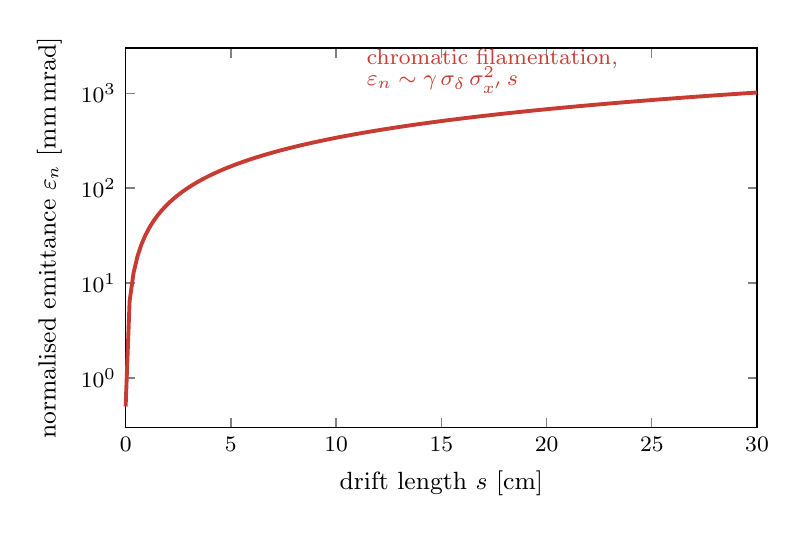
\begin{tikzpicture}

  \begin{axis}[
      width=9.6cm, height=6.4cm,
      xlabel={drift length $s$ [cm]},
      ylabel={normalised emittance $\varepsilon_n$ [mm\,mrad]},
      xmin=0, xmax=30,
      ymin=0.3, ymax=3000,
      ymode=log,
      log basis y=10,
      xtick={0,5,10,15,20,25,30},
      ytick={1, 10, 100, 1000},
      tick align=inside,
      major tick length=0.12cm,
      tick style={line width=0.5pt},
      axis line style={line width=0.6pt},
      label style={font=\small},
      tick label style={font=\footnotesize},
      enlargelimits=false,
      clip=false,
  ]

    % Chromatic growth (analytic Migliorati Eq. (5) in drift, parameters
    % tuned so that eps_n grows from ~0.5 to ~1000 mm.mrad over 30 cm,
    % matching the regime of Migliorati 2013 Fig. 2).
    % Functional form: eps_n(s) = sqrt( eps_0^2 + (k s)^2 ).
    \addplot[chromcurve, line width=1.4pt, domain=0:30, samples=160]
      {sqrt(0.5^2 + (34*x)^2)};

    % Inline label identifying the curve and the scaling law
    \node[font=\footnotesize, color=chromcurve, anchor=west, align=left] at
      (axis cs:11, 1700)
      {chromatic filamentation,\\[-2pt]
       $\varepsilon_n \sim \gamma\,\sigma_\delta\,\sigma_{x'}^2\,s$};

  \end{axis}

\end{tikzpicture}
\end{document}
